The results of the comparison of galaxy property values for TNG and SAMI are presented in this section. 

\subsection{Stellar to halo mass relation}
The SHM relation from TNG is plotted in Figure \ref{shmr_res}, along with the best fits from \textcite{Behroozi2013} and \textcite{Zanisi2019}. At low halo masses, the TNG galaxies have on average slightly higher stellar masses than \textcite{Behroozi2013}, but the difference is significant from \textcite{Zanisi2019}. The turn around point $M_1$ for TNG is similar to that of both abundance matching fits. For $M_{halo} > 10^{12} M_{\odot}$, the TNG SHM relation deviates significantly from the abundance matching fit by having a much steeper slope. This indicates a value for $\gamma$ in equation \ref{eq_behroozi} closer to unity. The more recent results from \textcite{Zanisi2019} agrees better with the high mass slope, but the difference is still significant. The deviation from observations is expected, as TNG has been found to produce galaxies with too high stellar mass in larger subhalos (//cite). This might indicate a too high star formation rate in these galaxies.


\begin{figure}
    \centering
    \makebox[\textwidth][c]{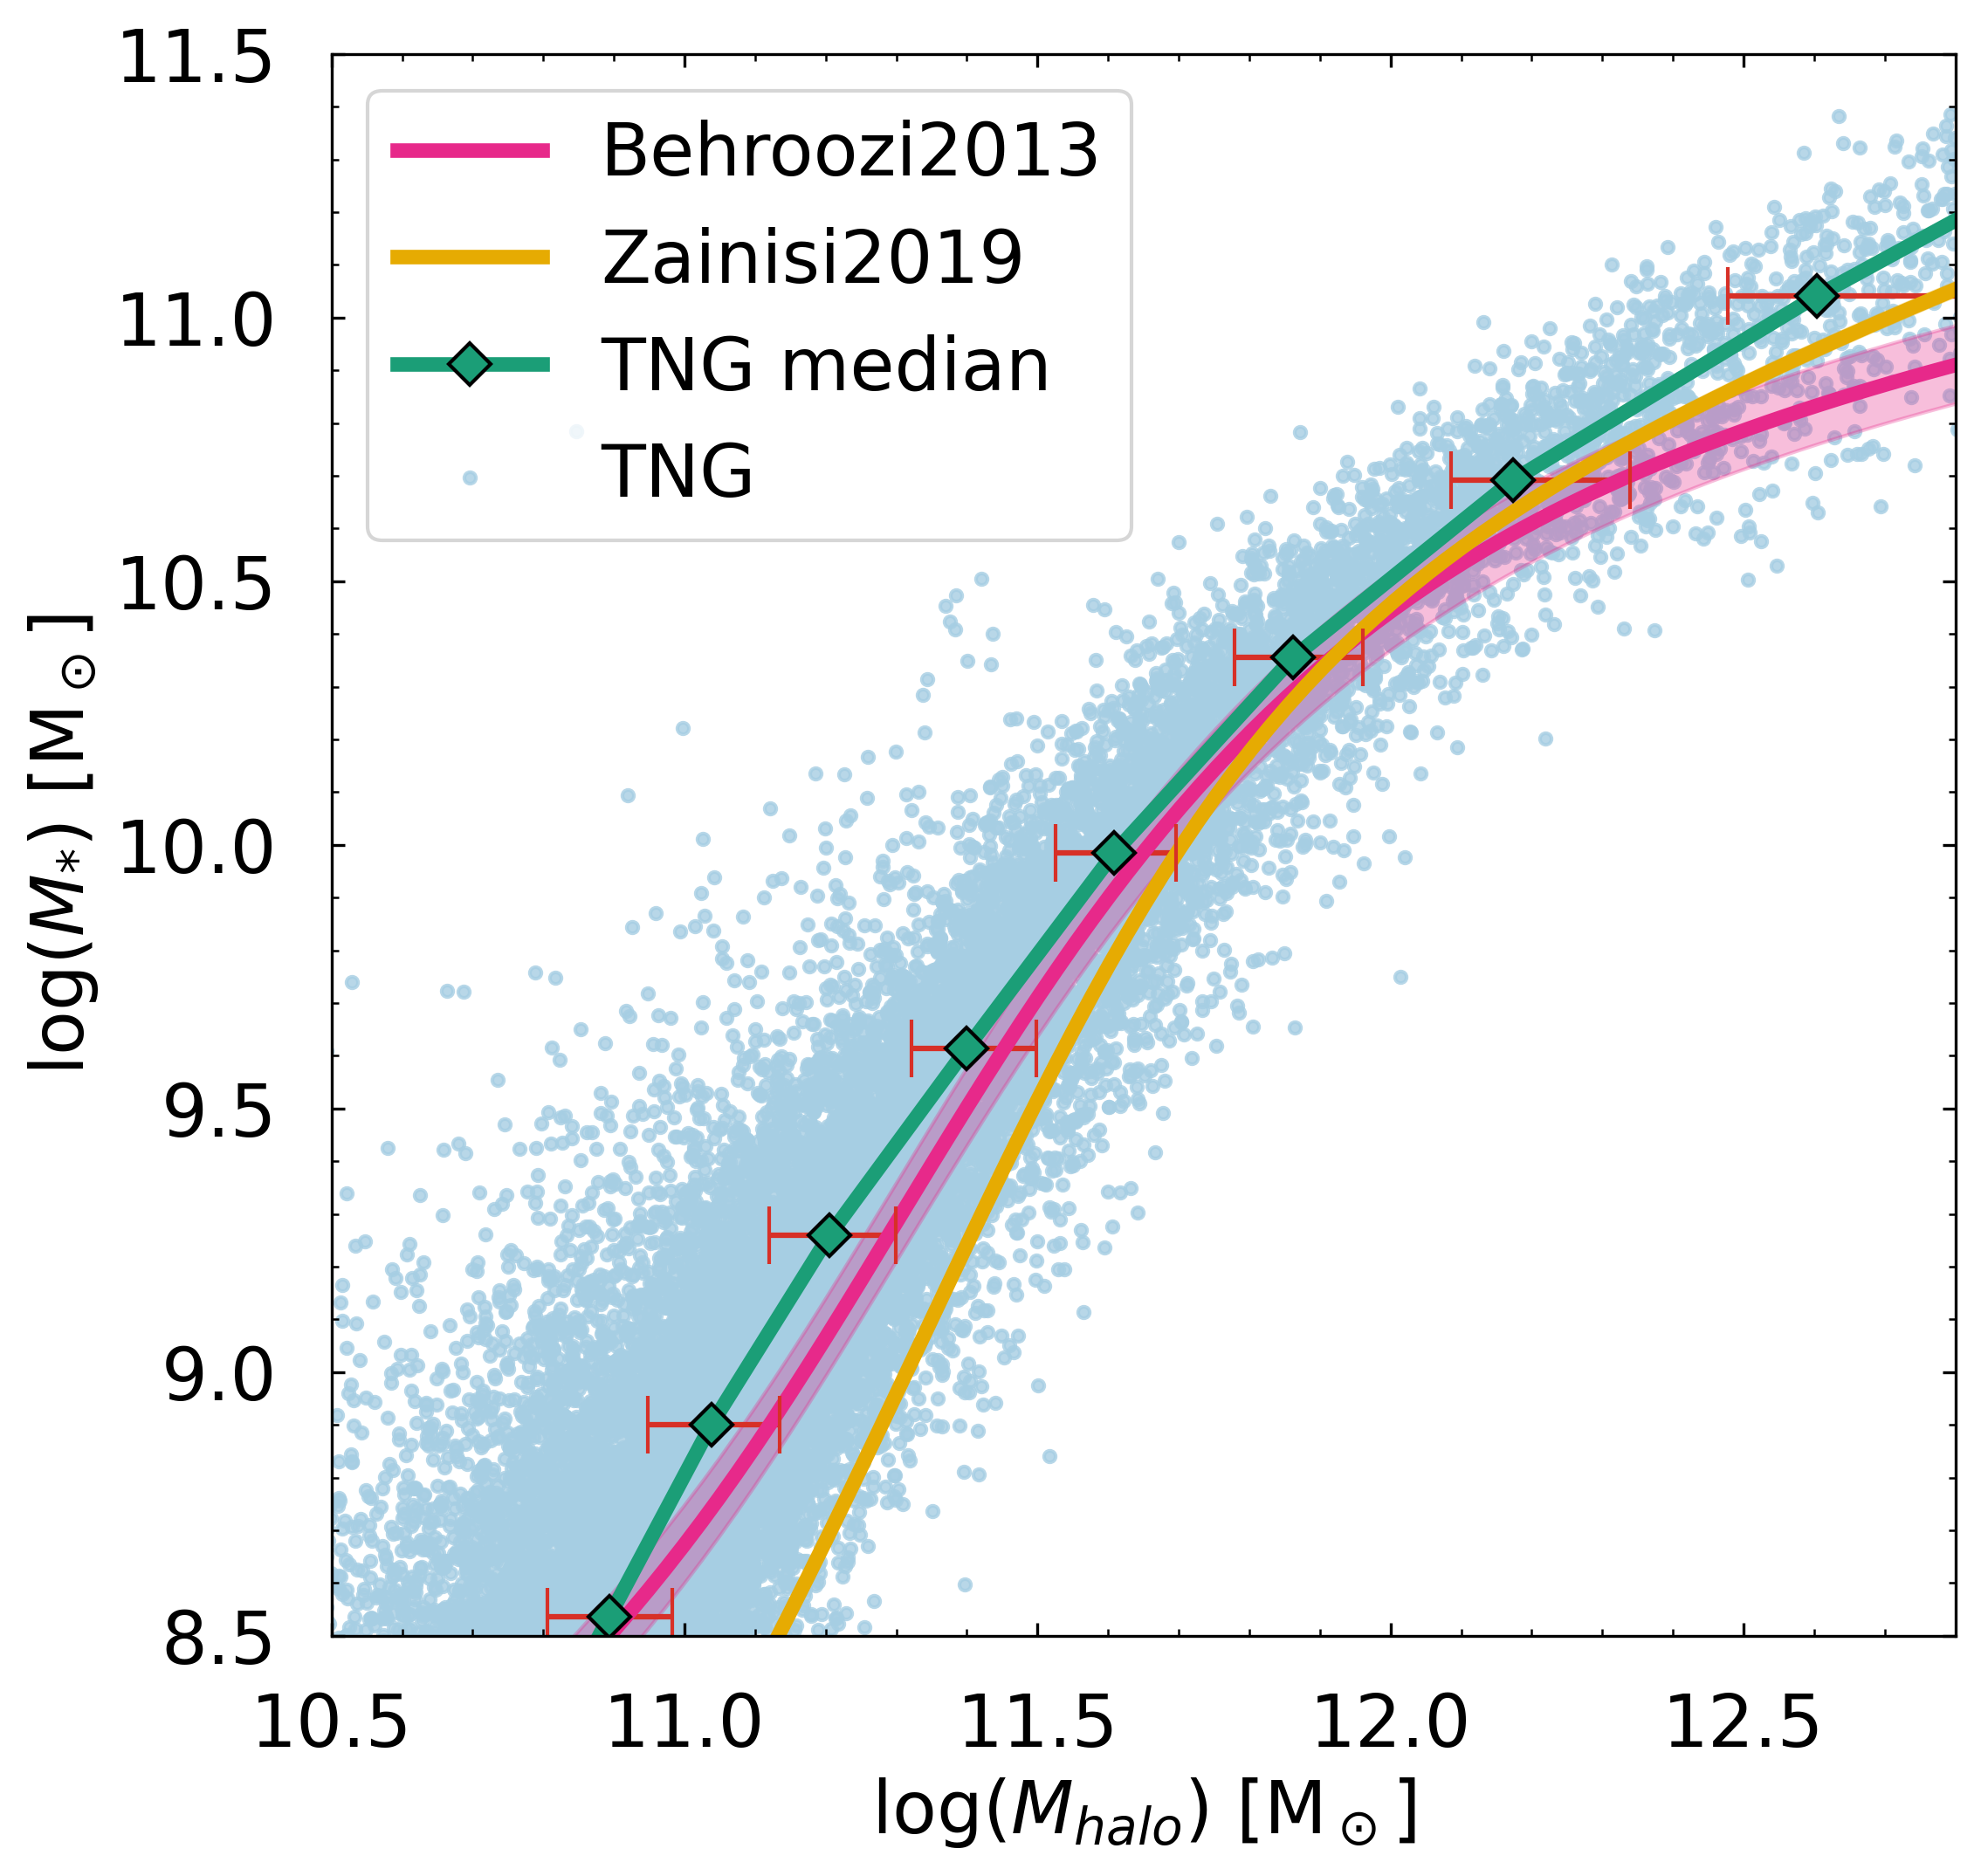
\includegraphics[width=0.7\textwidth]{images/results_shmr.png}}
    \caption{The SHM relation of TNG is shown (blue dots), along with median points (green markers) with error bars showing the 25-75 percentile. The best fit from abundance matching from \textcite{Behroozi2013} (pink dashed line) and \textcite{Zanisi2019} (yellow line)) are also shown.} 
    \label{shmr_res}
\end{figure}


\subsection{Tully-Fisher relation}
The TFR for the late type galaxies in TNG is shown in Figure \ref{tfr_res} along with the best fit for the SAMI data found in \textcite{Bloom2017}. The linear fit to TNG gives a slope of 4.13. This is steeper than that found for the SAMI data, which has a slope of 3.23. As massive TNG galaxies were found to have lower halo masses compared to data, this would also lead to lower velocity values, and might explain the difference in slope. Rotational velocities for TNG are chosen as the maximum velocity on the velocity curve, while \textcite{Bloom2017}. use the velocity at $r = 2.2 r_e$. A better comparison could be made by choosing the same definition for the rotational velocity for both data sets. This is something which could be explored in future work.

It might also be interesting to investigate the Baryonic Tuller-Fisher relation by adding the hydrogen gas mass and velocity measurements to the stellar measurements. 
%not clear

\begin{figure}
    \centering
    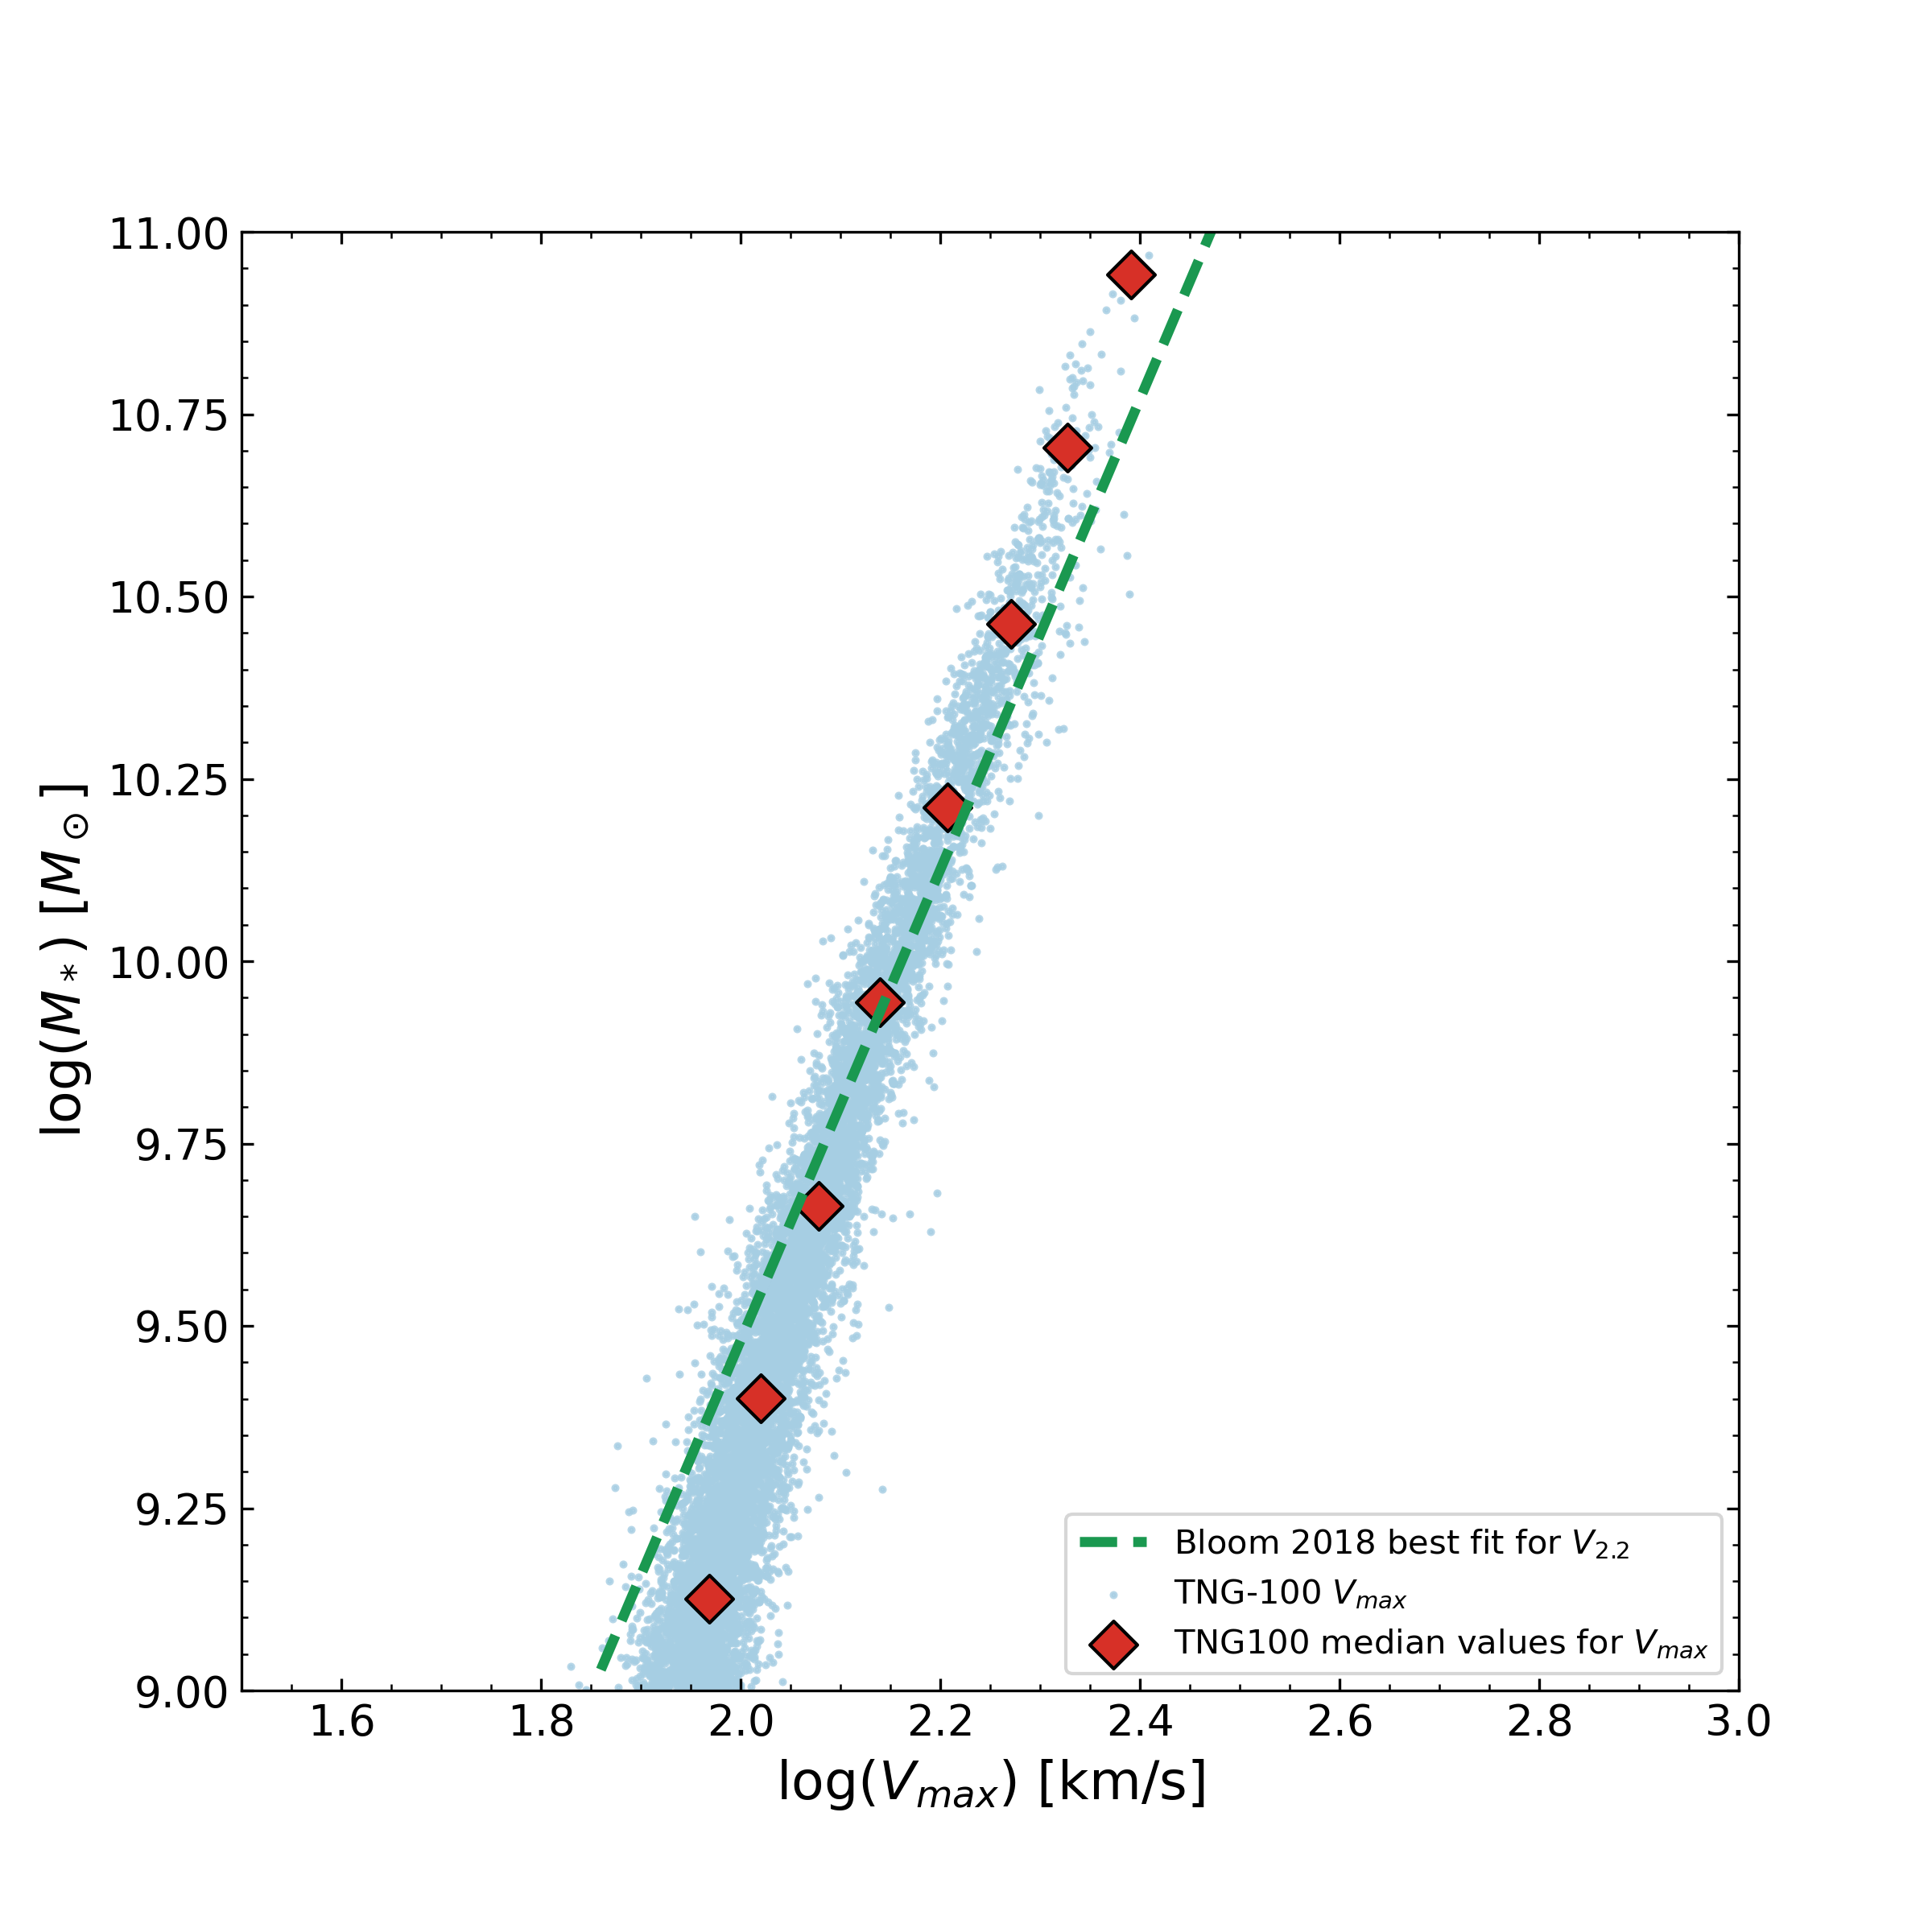
\includegraphics[width=0.7\textwidth]{images/results_tully_fisher.png}
    \caption{The TFR for TNG (blue dots). The median points for TNG are plotted with error bars, showing the 25-75 percentile. The TNG linear fit is also provided (blue line). The best fit for the SAMI data from \textcite{Bloom2017} is also shown (dashed line).}
    \label{tfr_res}
\end{figure}

\subsection{Faber Jackson relation and the fundamental plane}

The velocity dispersion as function of stellar mass (FJ relation) can be seen in Figure \ref{FJ_res}. The trend for the TNG data is a clear power law as expected. Using linear regression, the slope for TNG was found to be 3.14, with a zero-point of 4.21. Compared to the observational data, the simulation shows lower $\sigma$ values, by about 0.1-0.2 dex, while the slope is similar. The velocity dispersion in TNG galaxies is averaged across all particles identified by subfind while for SAMI, they are calculated from stars only and just in the inner part of the galaxy. In general, gas has a lower $\sigma$ than stars and dark matter, so this could push the total $\sigma$ down for TNG. However, in early-type galaxies there is little gas so the impact would be expected to be small. Other studies have also found that simulations tend to get lower values for $\sigma$ \parencite{Sande2018}, so this might be a limitation of the simulations.

%Another projection of the Fundamental Plane is the stelllar mass-radius relation....
The stellar mass-radius relation is shown in Figure \ref{FP_res1}. TNG has early type galaxies with smaller radius than SAMI. The radius for TNG is defined as the half mass radius, while SAMI uses half-light radius as described in section \ref{radius}. Half-light radius tends to be larger than half-mass radius \parencite{Sande2018}. Apart from this, the general trend of the relation is similar in both data sets.

The $\sigma$-radius relation can be seen in Figure \ref{FP_res2}. This relation is also affected by the systematically lower $\sigma$ values for TNG, as well as the lower radii. The scatter in the data is comparatively large for both TNG and SAMI.

For the mass-radius and $\sigma$-radius relations it would be interesting to calculate the half-light radius for TNG instead of using the half-mass radius (this has been done for instance by \textcite{Genel2017}). This could be studied in future work, along with choosing the same method of calculating the velocity dispersion for simulation and observation data.

\begin{figure}
    \centering
    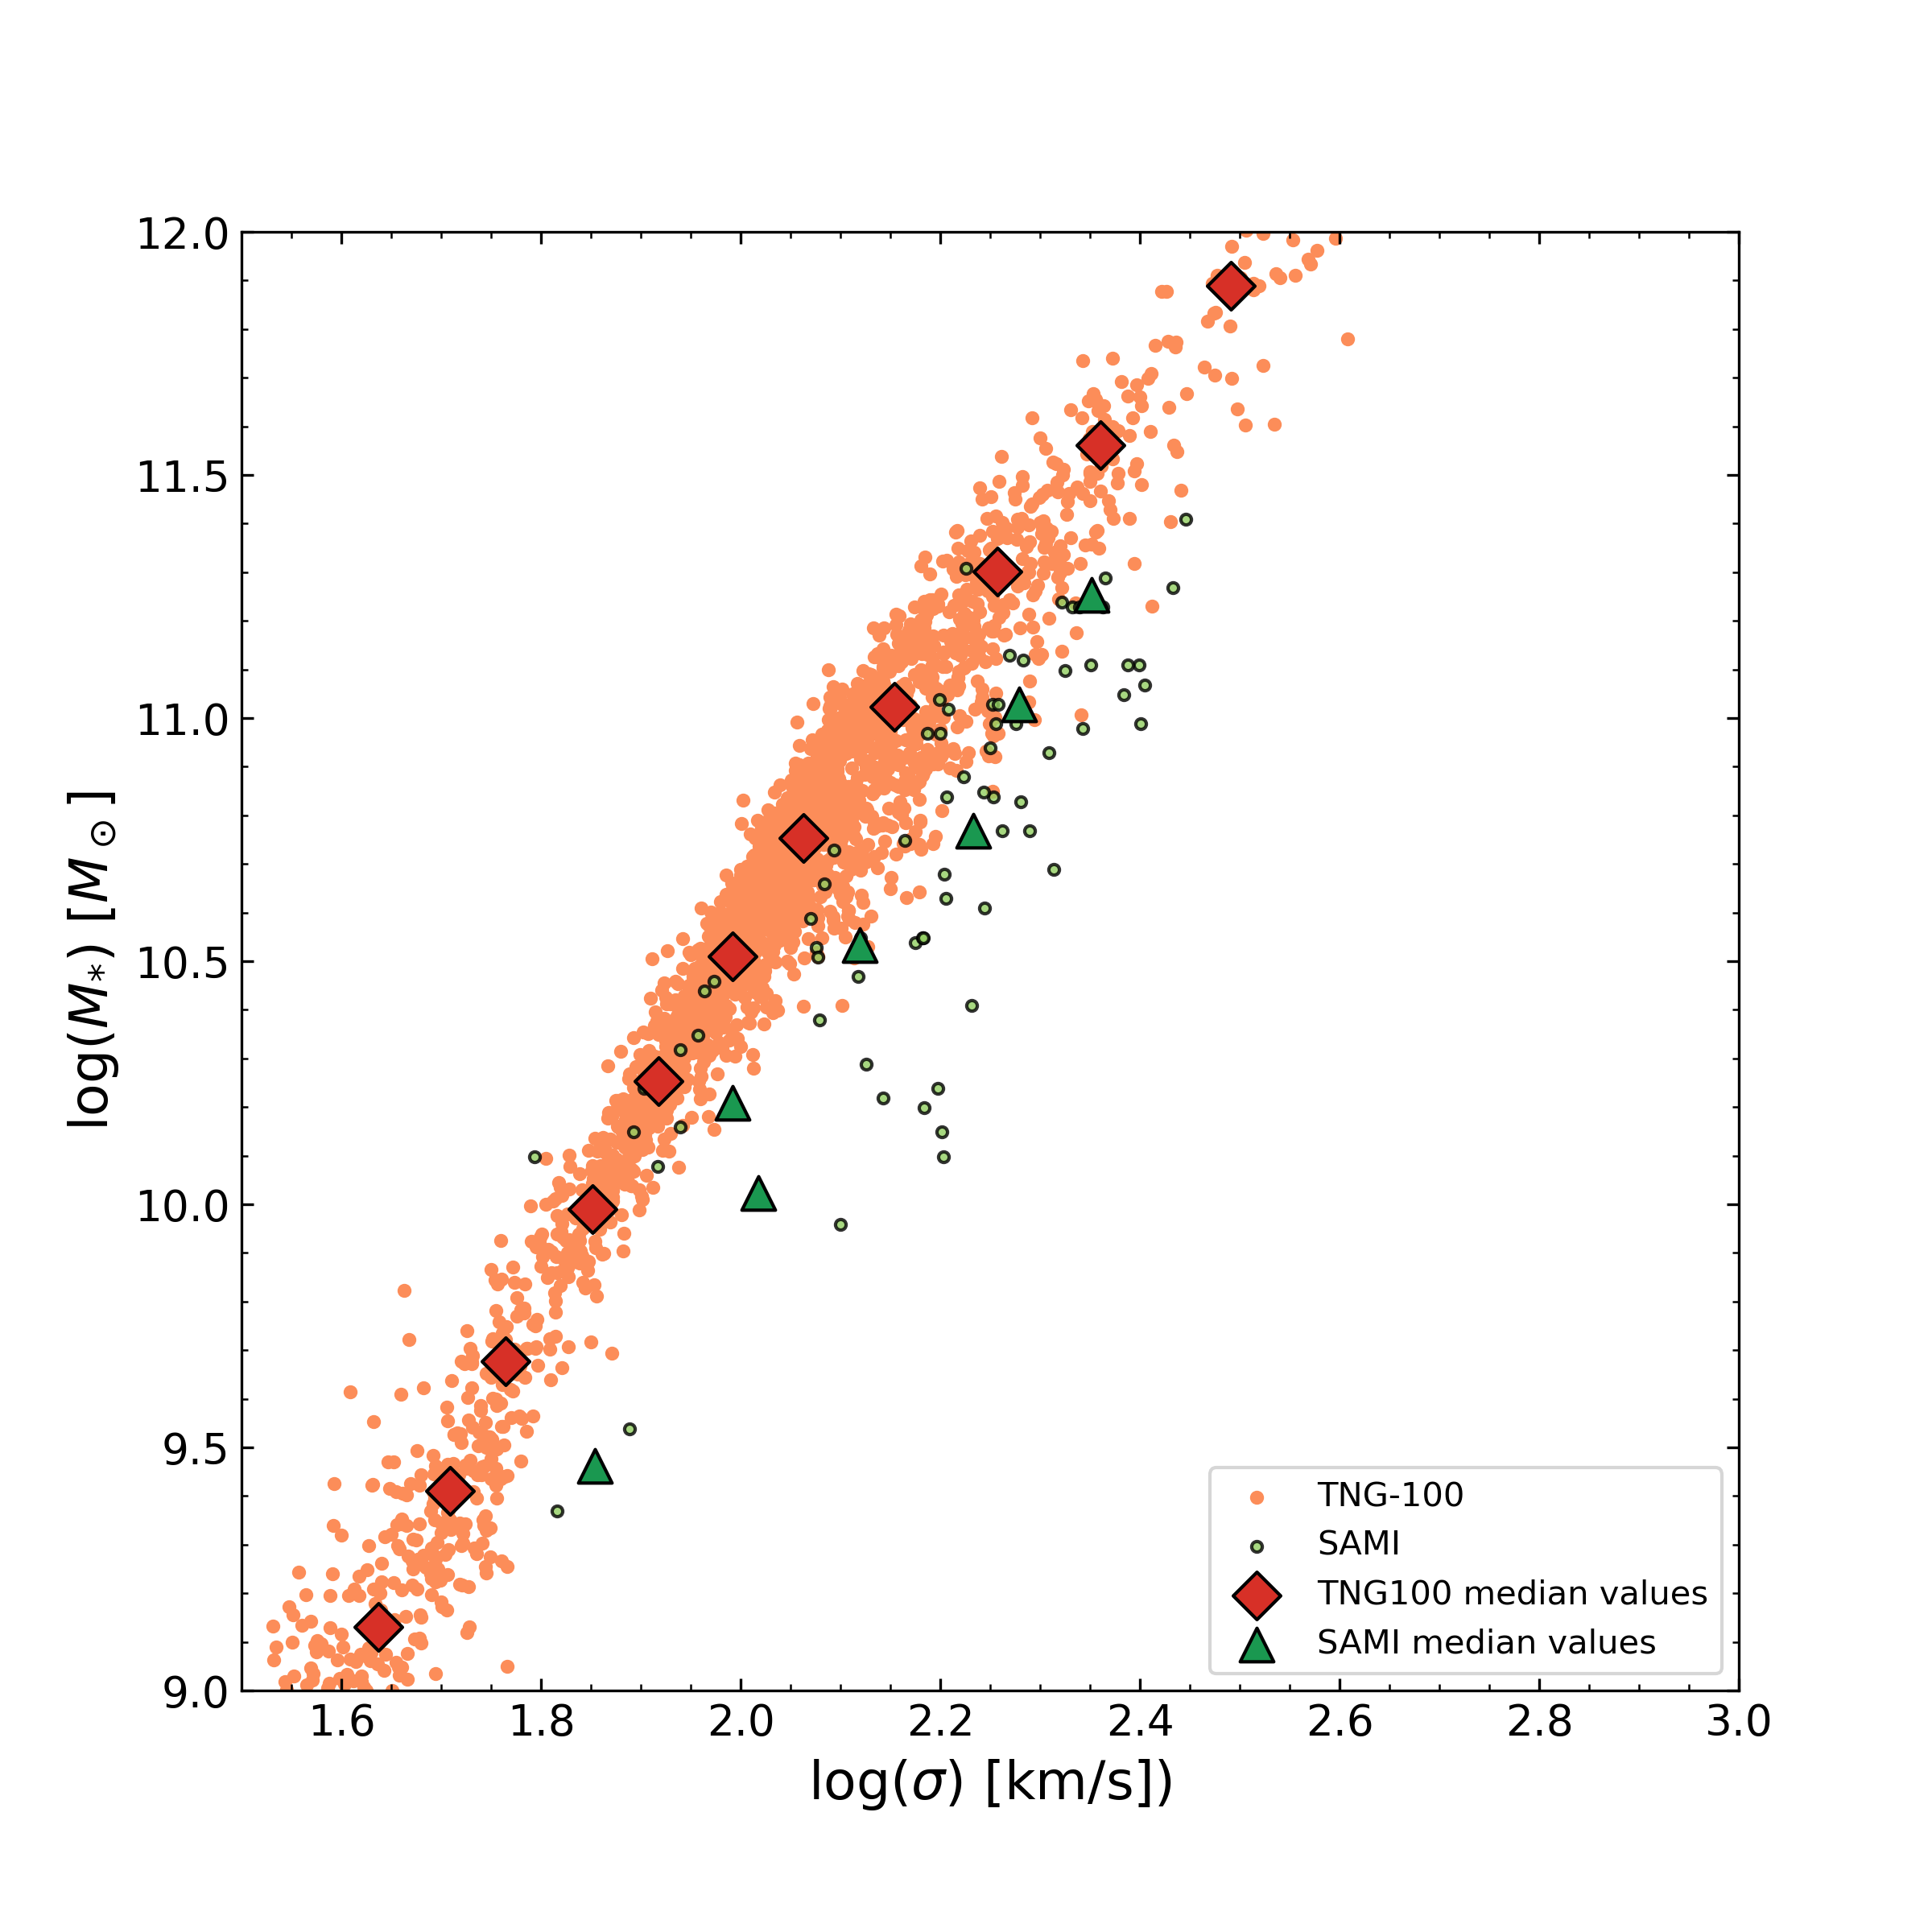
\includegraphics[width=0.7\textwidth]{images/results_faber_jackson.png}
    \caption{The FJ relation in early type galaxies for TNG (red dots) and SAMI (green dots). The median values with 25-75 percentile error bars are also shown. For SAMI, the median values are not calculated below a stellar mass of $10^10 M_\odot$. The linear fit to the TNG data is shown as a solid red line, and has a slope of 3.14 with a zero-point of 4.2.}
    \label{FJ_res}
\end{figure}

\begin{figure}
    \centering
    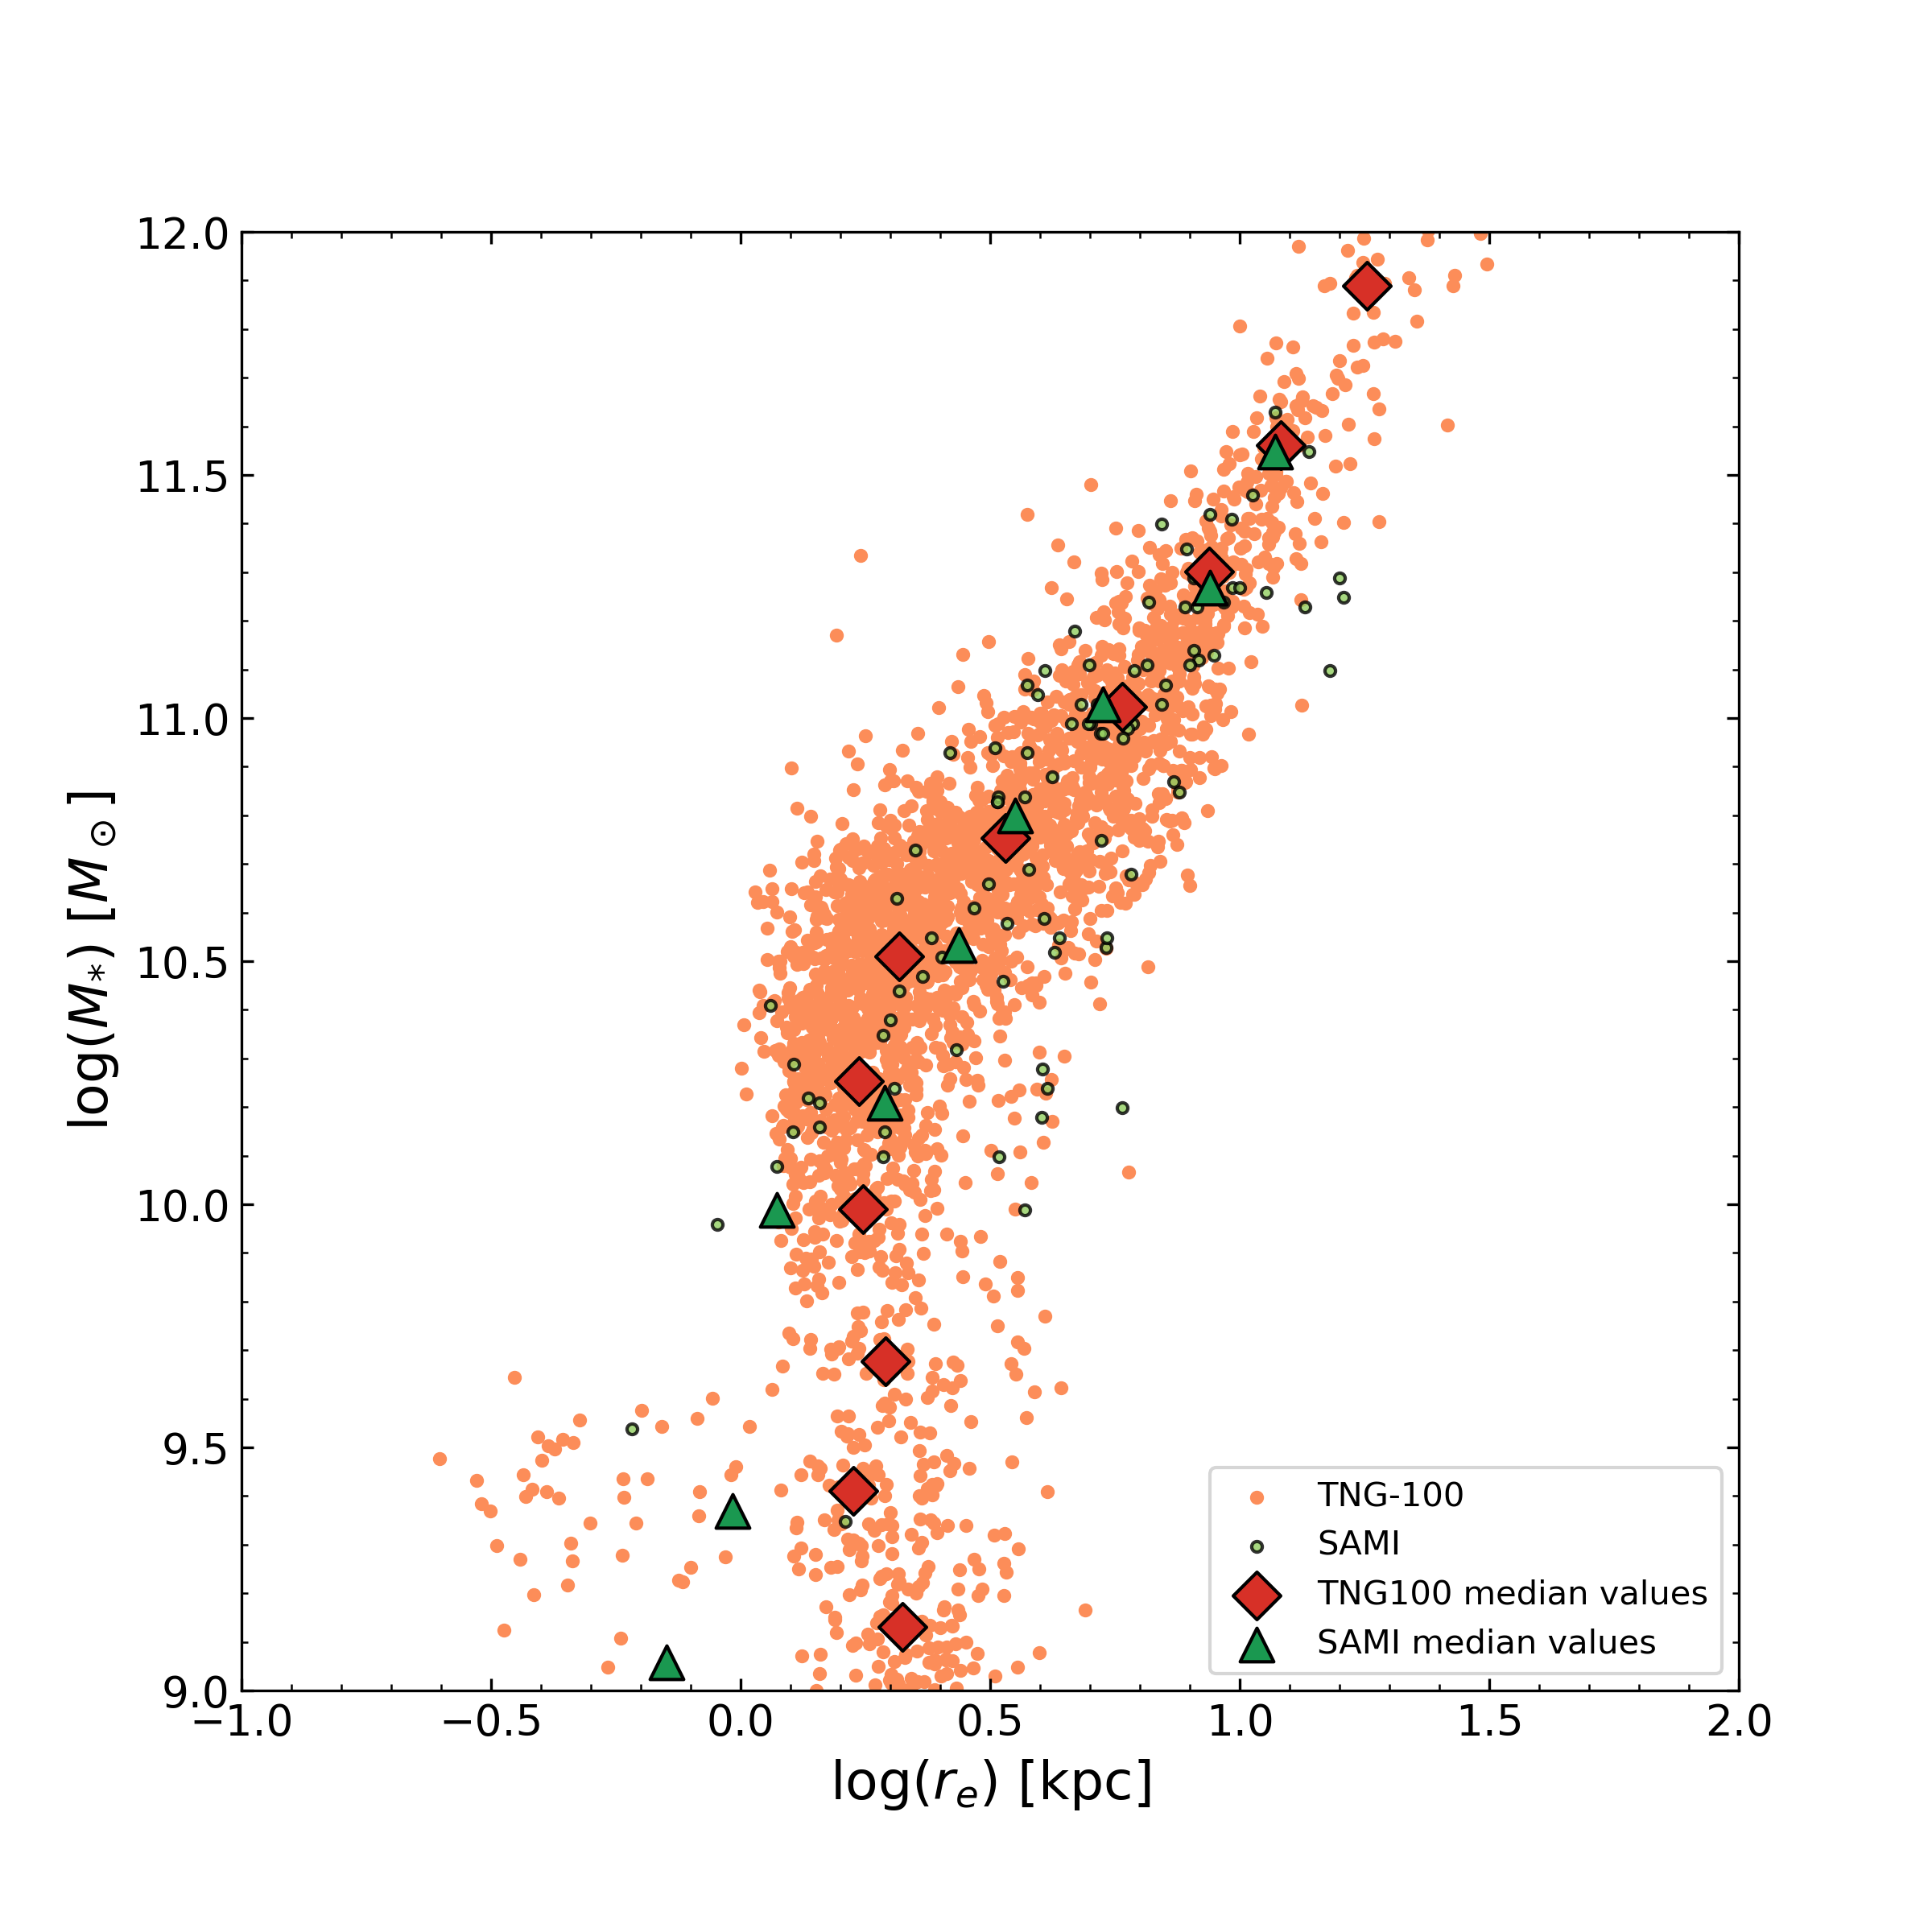
\includegraphics[width=0.7\textwidth]{images/results_mass_radius_FP.png}
    \caption{The stellar mass as a function of effective radius in early type galaxies for TNG (red dots) and SAMI (green dots). Median values are also shown with 25-75 percentile error bars. SAMI median values are only calculated for masses above $M_* = 10^{9.7} M_\odot$ as there are too few data points below this mass.}
    \label{FP_res1}
\end{figure}

\begin{figure}
    \centering
    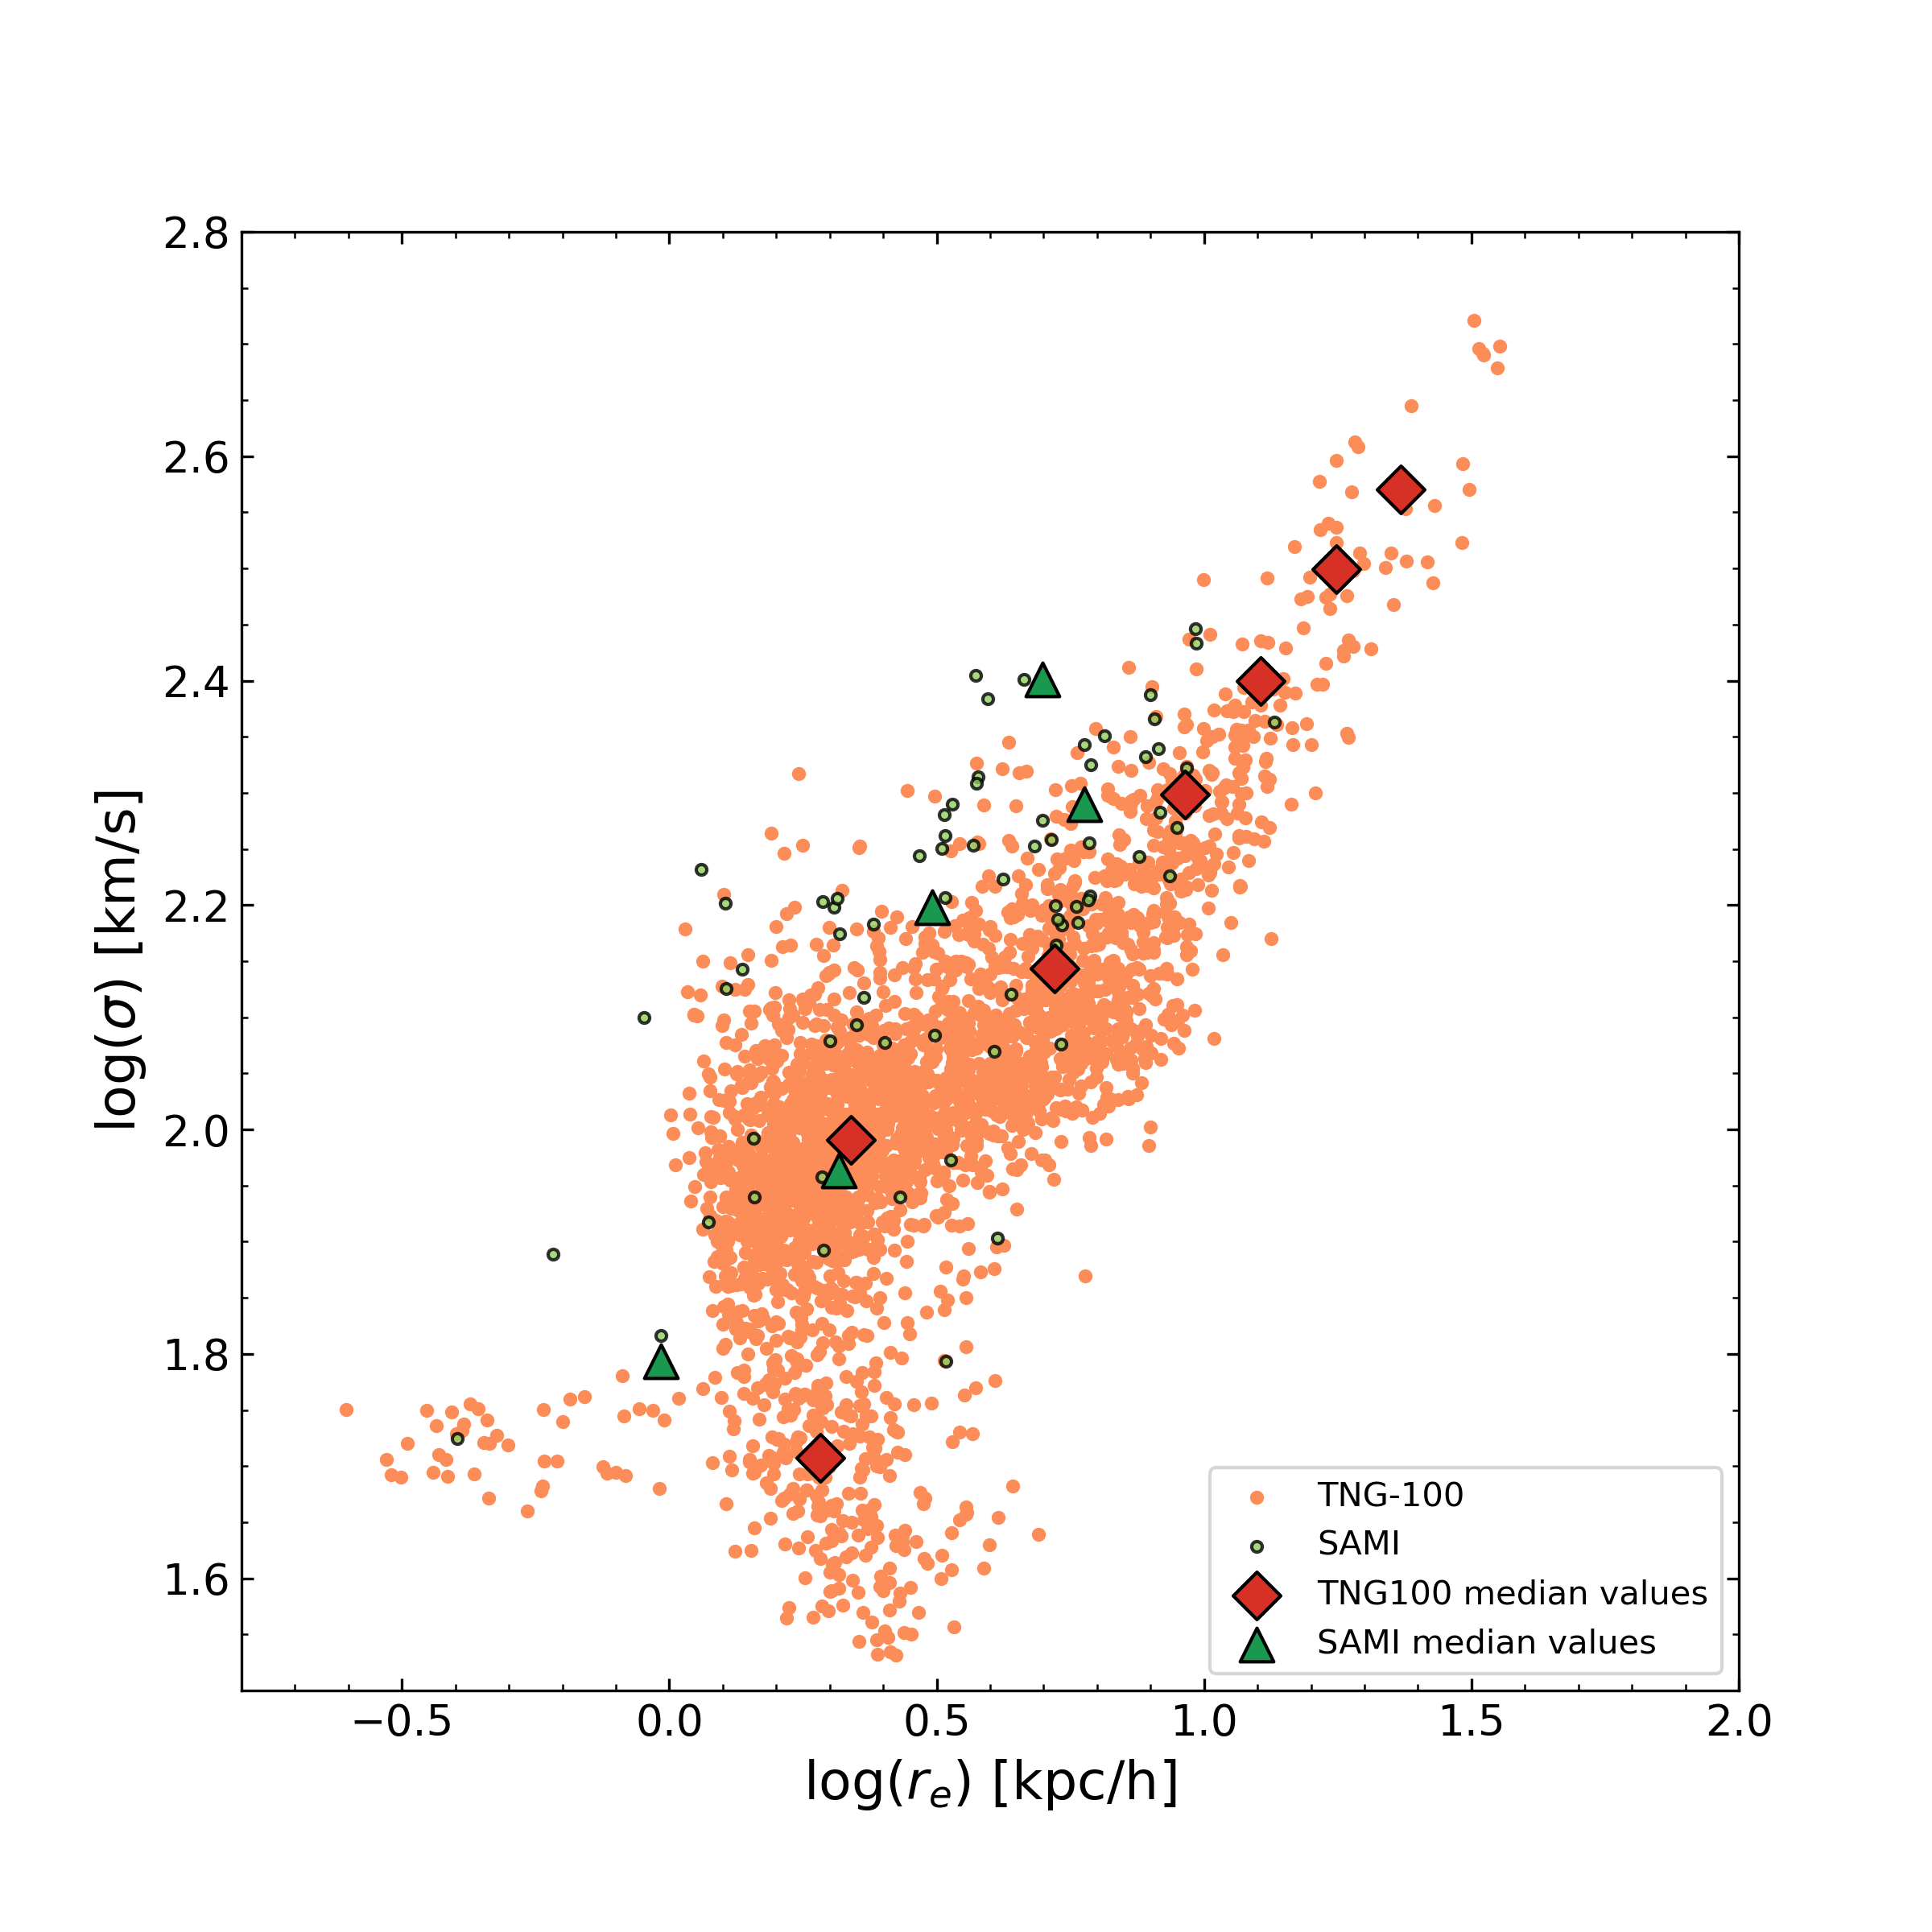
\includegraphics[width=0.7\textwidth]{images/results_sigma_radius_FP.png}
    \caption{Velocity dispersion as a function of effective radius for early type galaxies for TNG (red dots) and SAMI (green dots). Also included are median values and 25-75 percentile error bars for both data sets.}
    \label{FP_res2}
\end{figure}

\newpage

\subsection{Color bimodality}
The g-i color-mass diagrams for TNG and SAMI are shown in Figure \ref{color_magnitude_res}. There is a distinct seperation between early and late type galaxies in TNG, as expected. For SAMI, the distinction is less clear. The early type galaxies in SAMI are redder than the late type galaxies on average, but there is a significant amount of late type galaxies with similar mass and color as the early types. Interestingly enough, it has been noted by other work that TNG produces too many red late type galaxies compared to observations \parencite{Nelson2017}, but in this case we get the opposite effect. This might have to do with the different classification method of early and late type galaxies in SAMI and TNG. In general, the SAMI galaxies are also on average redder than the TNG galaxies. \textcite{Nelson2017} found the color bimodality in TNG to generally be in good agreement with observations despite the larger amount of red late type galaxies, and notes a large improvement with respect to the original Illustris simulation.


In Figure \ref{pdf_color} the PDF for the TNG and SAMI g-i colors are shown. The peaks coincide well for the two data sets, but the slight shift towards redder values for SAMI is apparent here also. The SAMI late type galaxy distribution has a peak, but it is not as profound as for TNG. If galaxies with mass down to $10^8 M_{\odot}$ are included for SAMI, the peak becomes much more profound, so in future work it would be interesting to look at TNG data for galaxies with smaller stellar masses as well. It is worth noting that TNG has a distribution of early type galaxies with an extra ``bump'' towards the blue end of the spectrum, while SAMI has a bump on the late type galaxy distribution. This is also something which could be studied in further work. 
\begin{figure}
    \centering
    \makebox[\textwidth][c]{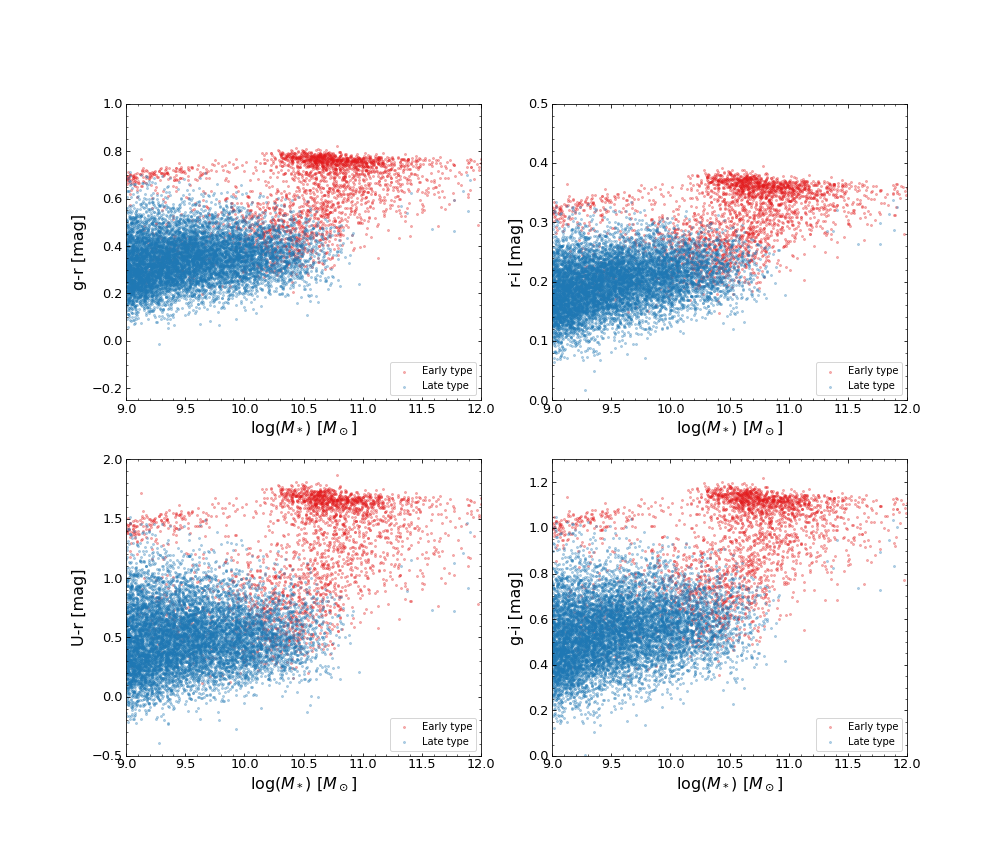
\includegraphics[width=1.1\textwidth]{images/results_color_magnitude.png}}
    \caption{Left: TNG g-i color-mass diagram. Late type and early type galaxies are shown in different colors, blue and red respectively. Right: SAMI g-i color-mass diagram with early type (red) and late type galaxies (blue) plotted seperately.}
    \label{color_magnitude_res}
\end{figure}


\begin{figure}
    \centering
    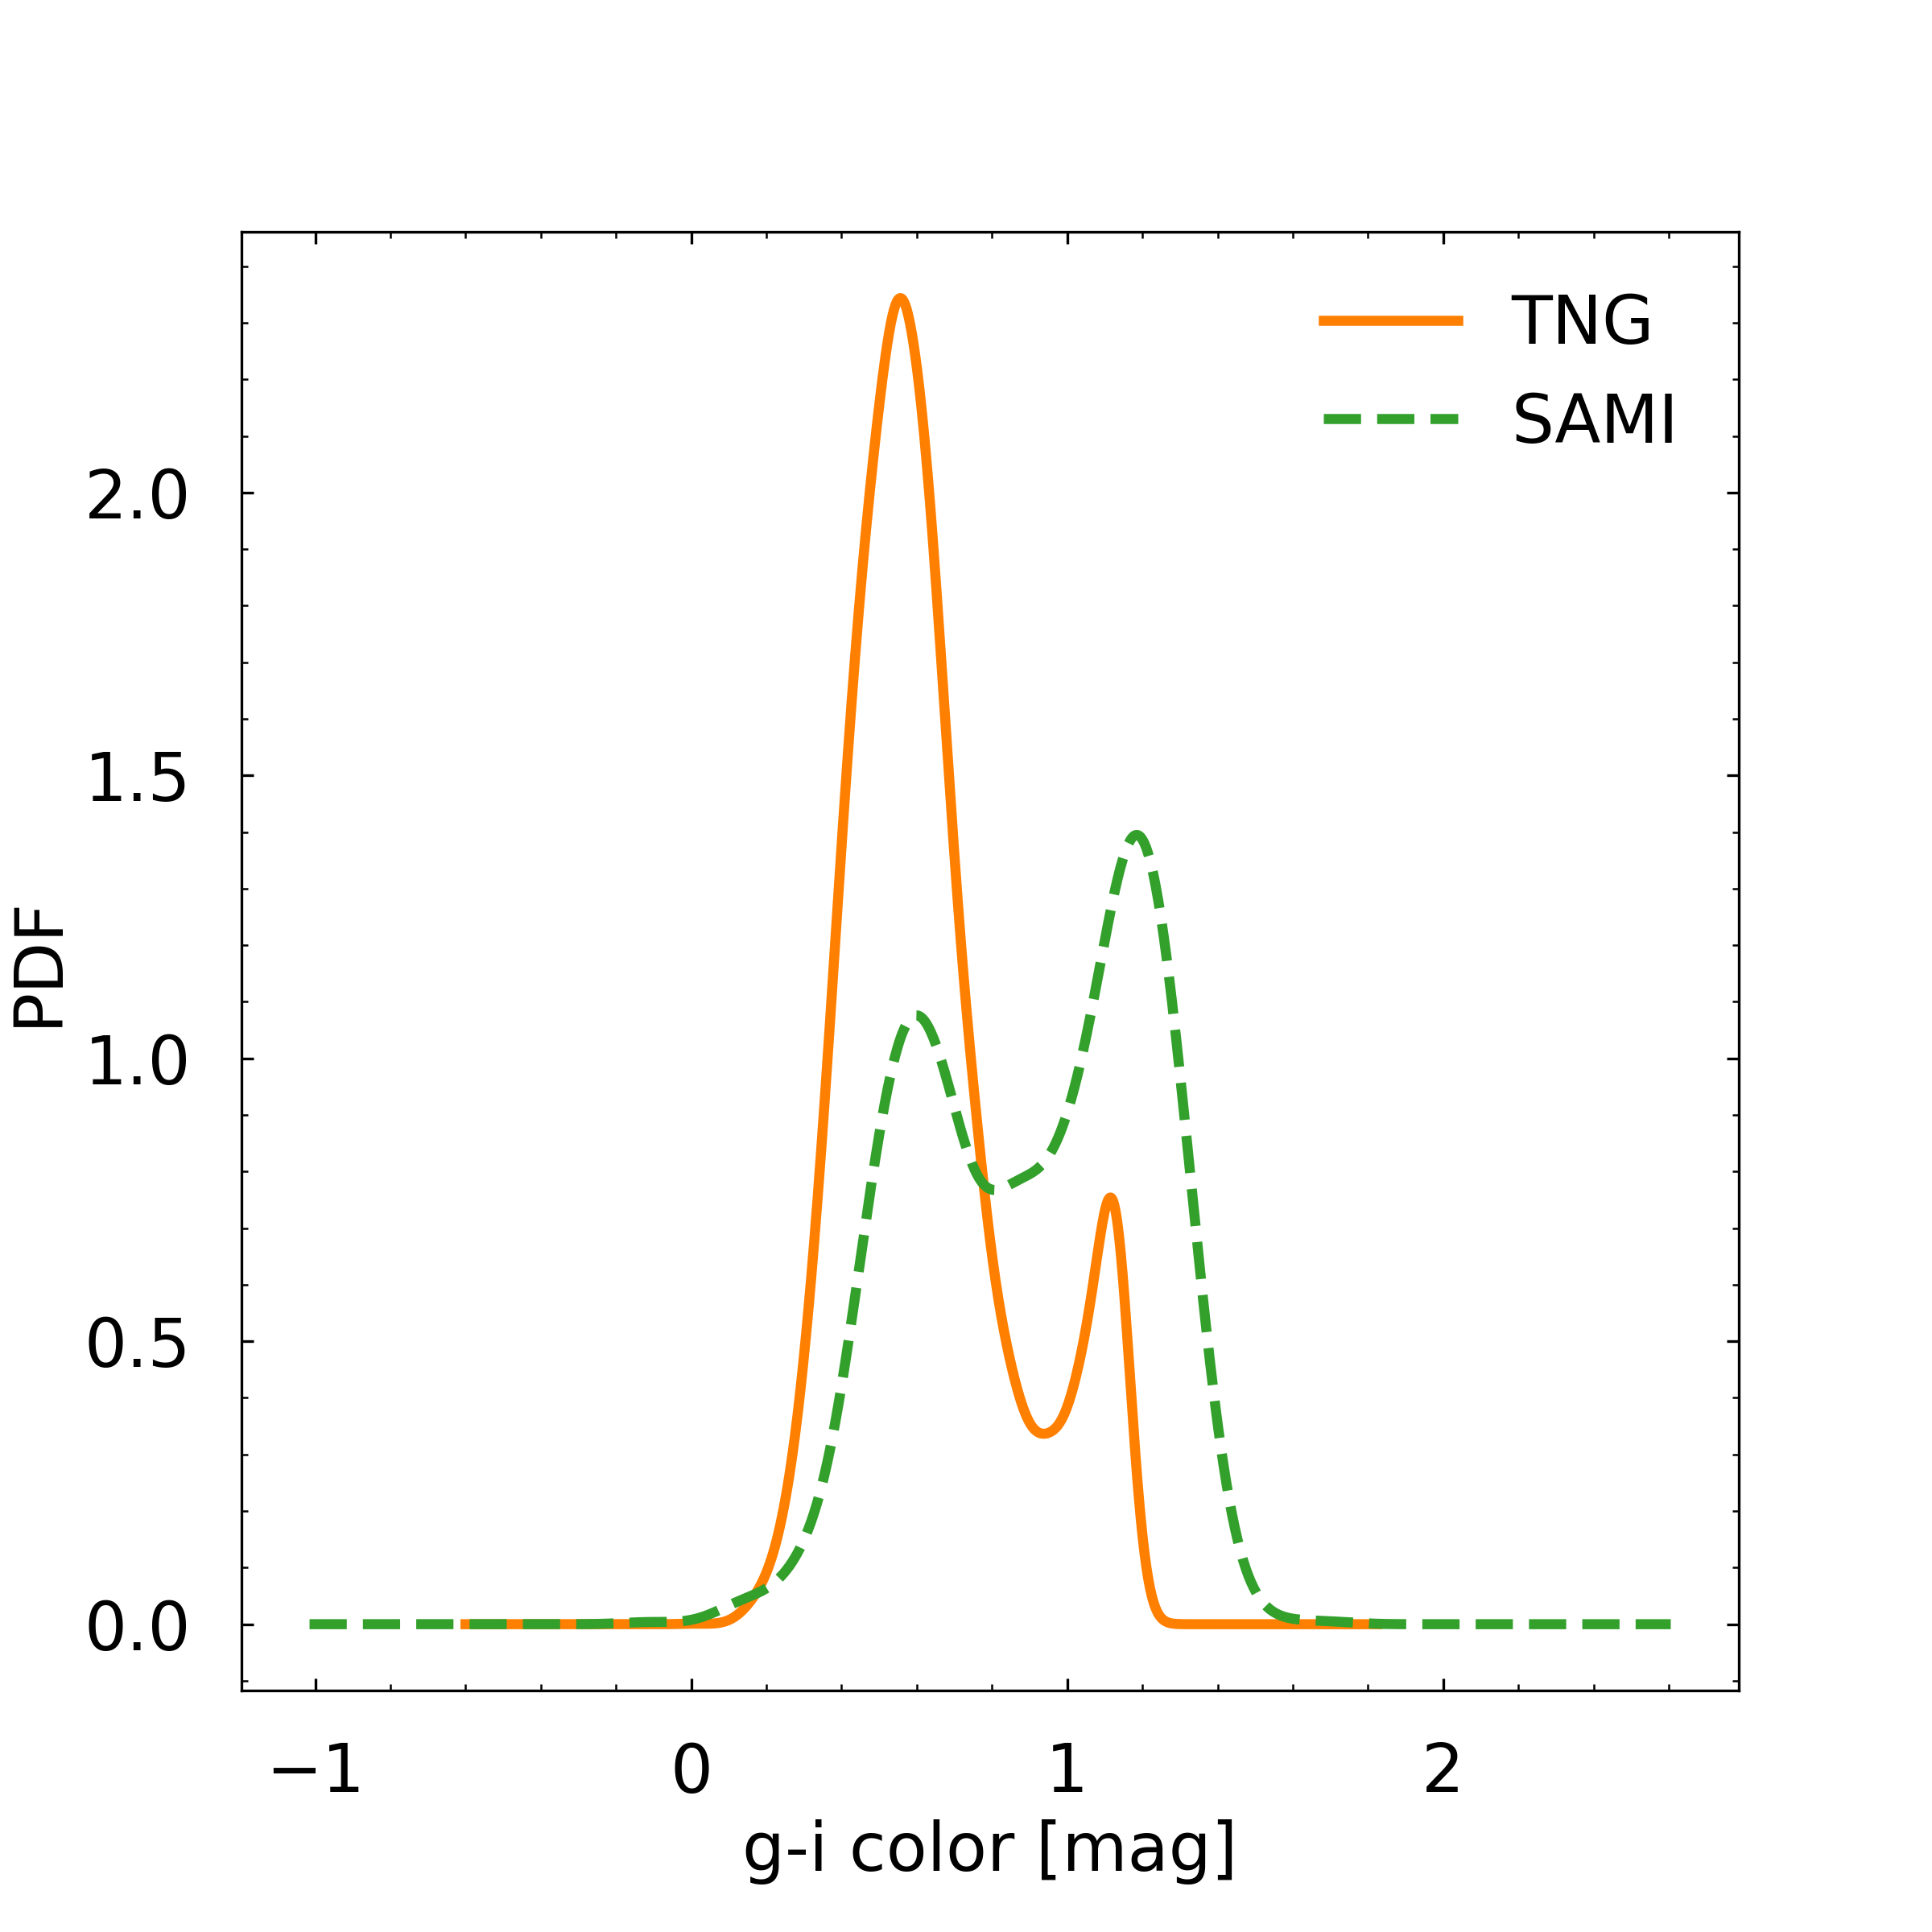
\includegraphics[width=0.7\textwidth]{images/results_pdf_g_i_band.png}
    \caption{The distribution of g-i color in TNG and SAMI. Kernel density weighted PDF (with Gaussian kernels) are shown for TNG early and late types (red and blue solid lines) as well as for SAMI (red and blue dashed lines). The values are not normalized, so the height of the peak is not comparable, but the x-position and width is.}
    \label{pdf_color}
\end{figure}

